% =============================================================================
% 5.6 集成层端到端任务完成率评测
% 草稿版本：v0.2 (2026-05-07)
%   v0.1：作为 5.2.5 子小节起草。
%   v0.2：按导师意见 3 提级为 5.6 \subsection；首段"前 4 节的模块层评测"
%        改为对应新结构 5.2--5.5 节的措辞。
% 字数：约 1500 字
% 风格规则：v0.2 风格（无 \textbf / \textit / 引例括号 / 双引号 / 破折号）
% 引用：\cite{ref1, ref18, ref20}
% 图表：
%   - 表 \reftab{tab:e2e-overall}        双档 5 类断言总表
%   - 表 \reftab{tab:e2e-by-category}    按场景类别拆分
%   - 图 \reffig{fig:e2e-by-category}    6 类场景双档对比柱状图（含差距标注）
% 复用 4.3 节已有图表：\reftab{tab:report-judge-summary}
% 依赖宏包：booktabs / tabularx / graphicx（主稿已加载）
% =============================================================================

\subsection{集成层端到端任务完成率评测}
\label{sec:e2e-eval}

前面 4 节的模块层评测已经分别量化了意图识别、混合检索、语义桥接
与代码执行 4 个子模块的能力上限。但单模块成绩好不一定端到端就好：
通路 B 单测层面 \texttt{citation} 真实性 100\%，集成到 ReAct 循环最后
报告生成阶段仍可能因为大语言模型在最终输出时省略 GB/T 编号而衰减。
这种集成衰减效应是单模块评测无法捕捉的盲区，必须以最终用户体验视角
进行集成层评测才能补足。本节即对应这一空白。

评测集 \texttt{e2e\_\bk{}bench.\bk{}jsonl} 共 30 条用例，覆盖 6 类真实场景：
单城市单要素的 \texttt{simple\_\bk{}query} 5 条、多城市对比的
\texttt{multi\_\bk{}compare} 5 条、一周温度或降水的 \texttt{trend\_\bk{}analysis}
5 条、找最热最冷或最大降水的 \texttt{extreme\_\bk{}search} 5 条、户外洗车
带伞跑步等的 \texttt{decision\_\bk{}support} 6 条、以及暴雨严寒台风等的
\texttt{warning\_\bk{}extreme} 4 条。所有用例完全基于真实和风天气与
Open-Meteo API 的实时数据，未使用合成数据。评测断言全部使用结构性
证据，例如必须包含温度数值、必须给出具体日期、必须出现 GB/T 编号等，
不依赖具体数值，保证可重复性。

实验设计为 \texttt{full} 与 \texttt{ablated} 双档对照。两档共享同一个
被测大语言模型 GLM-5.1（温度 0）、同一份意图识别加参数补全前置流程、
同一份 9 个气象 API 工具，关键差异仅在于 \texttt{full} 档保留双通路
RAG 强制规则与 \texttt{search\_\bk{}knowledge}、\texttt{bridge\_\bk{}weather\_\bk{}data}
两个 RAG 工具，\texttt{ablated} 档把上述工具与 system prompt 中的双
通路 RAG 规则全部删除，模拟普通工程师不做双通路 RAG 时的常规做法。
这种切分构造了一个干净的双通路 RAG 端到端价值的对照实验，不掺杂工具
调用能力或上下文理解差异。

评测指标包含 5 类断言加 1 项 LLM-as-judge 4 维度评分。5 类断言分别为
\texttt{key\_\bk{}facts} 关键事实点召回、\texttt{citation} 权威标准引用、
\texttt{grading} 规范气象分级词使用、\texttt{advice} 决策建议给出、
\texttt{judge\_\bk{}score} 4 维度综合分。端到端通过条件是
\texttt{key\_\bk{}facts} 召回率 $\geq 0.8$、按用例条件断言 \texttt{citation}
或 \texttt{grading} 或 \texttt{advice} 通过、且 \texttt{judge\_\bk{}overall}
分数 $\geq 3.0$。LLM-as-judge 4 维度的 Judge 模型与被测模型独立，按
事实性、完整性、专业性、流畅性四个 0 至 5 区间维度独立打分。30 条
用例双档对照的核心结果见 \reftab{tab:e2e-overall}。

\begin{table}[H]
    \centering
    \caption{端到端评测双档 5 类断言总表（30 条用例）}
    \label{tab:e2e-overall}
    \song\fontsize{9pt}{12pt}\selectfont
    \renewcommand{\arraystretch}{0.95}
    \begin{tabular}{lccc}
        \toprule
        指标 & ablated & full & 差距 \\
        \midrule
        端到端通过率 & 73.3\% & 86.7\% & $+13.4$ pp \\
        关键事实点召回率 & 99.2\% & 99.2\% & 持平 \\
        权威标准引用率 & 0.0\% & 26.7\% & $+26.7$ pp \\
        规范分级词出现率 & 100.0\% & 96.7\% & $-3.3$ pp \\
        决策建议出现率 & 90.0\% & 83.3\% & $-6.7$ pp \\
        Judge 综合分（0--5） & 4.27 & 4.31 & $+0.04$ \\
        平均工具调用次数 & 3.67 & 4.57 & $+0.90$ \\
        \bottomrule
    \end{tabular}
\end{table}

按场景类别拆分见 \reftab{tab:e2e-by-category}，对应可视化对比见
\reffig{fig:e2e-by-category}。差距最大的两类是
\texttt{decision\_\bk{}support} 与 \texttt{warning\_\bk{}extreme}：决策类
\texttt{ablated} 档通过率仅 50\%，\texttt{full} 档为 100\%，差距 50
个百分点；预警类 \texttt{ablated} 档为 50\%，\texttt{full} 档为 75\%，
差距 25 个百分点。简单查询、多城市对比、趋势分析与极值检索四类场景
两档持平。这一分布揭示一个具体规律：当问题需要权威标准支撑作为决策
依据时双通路 RAG 价值最大，当问题只需要信息检索本身时双通路 RAG 不
带来端到端通过率差异，但仍提供权威可溯源性。

\begin{figure}[!ht]
    \centering
    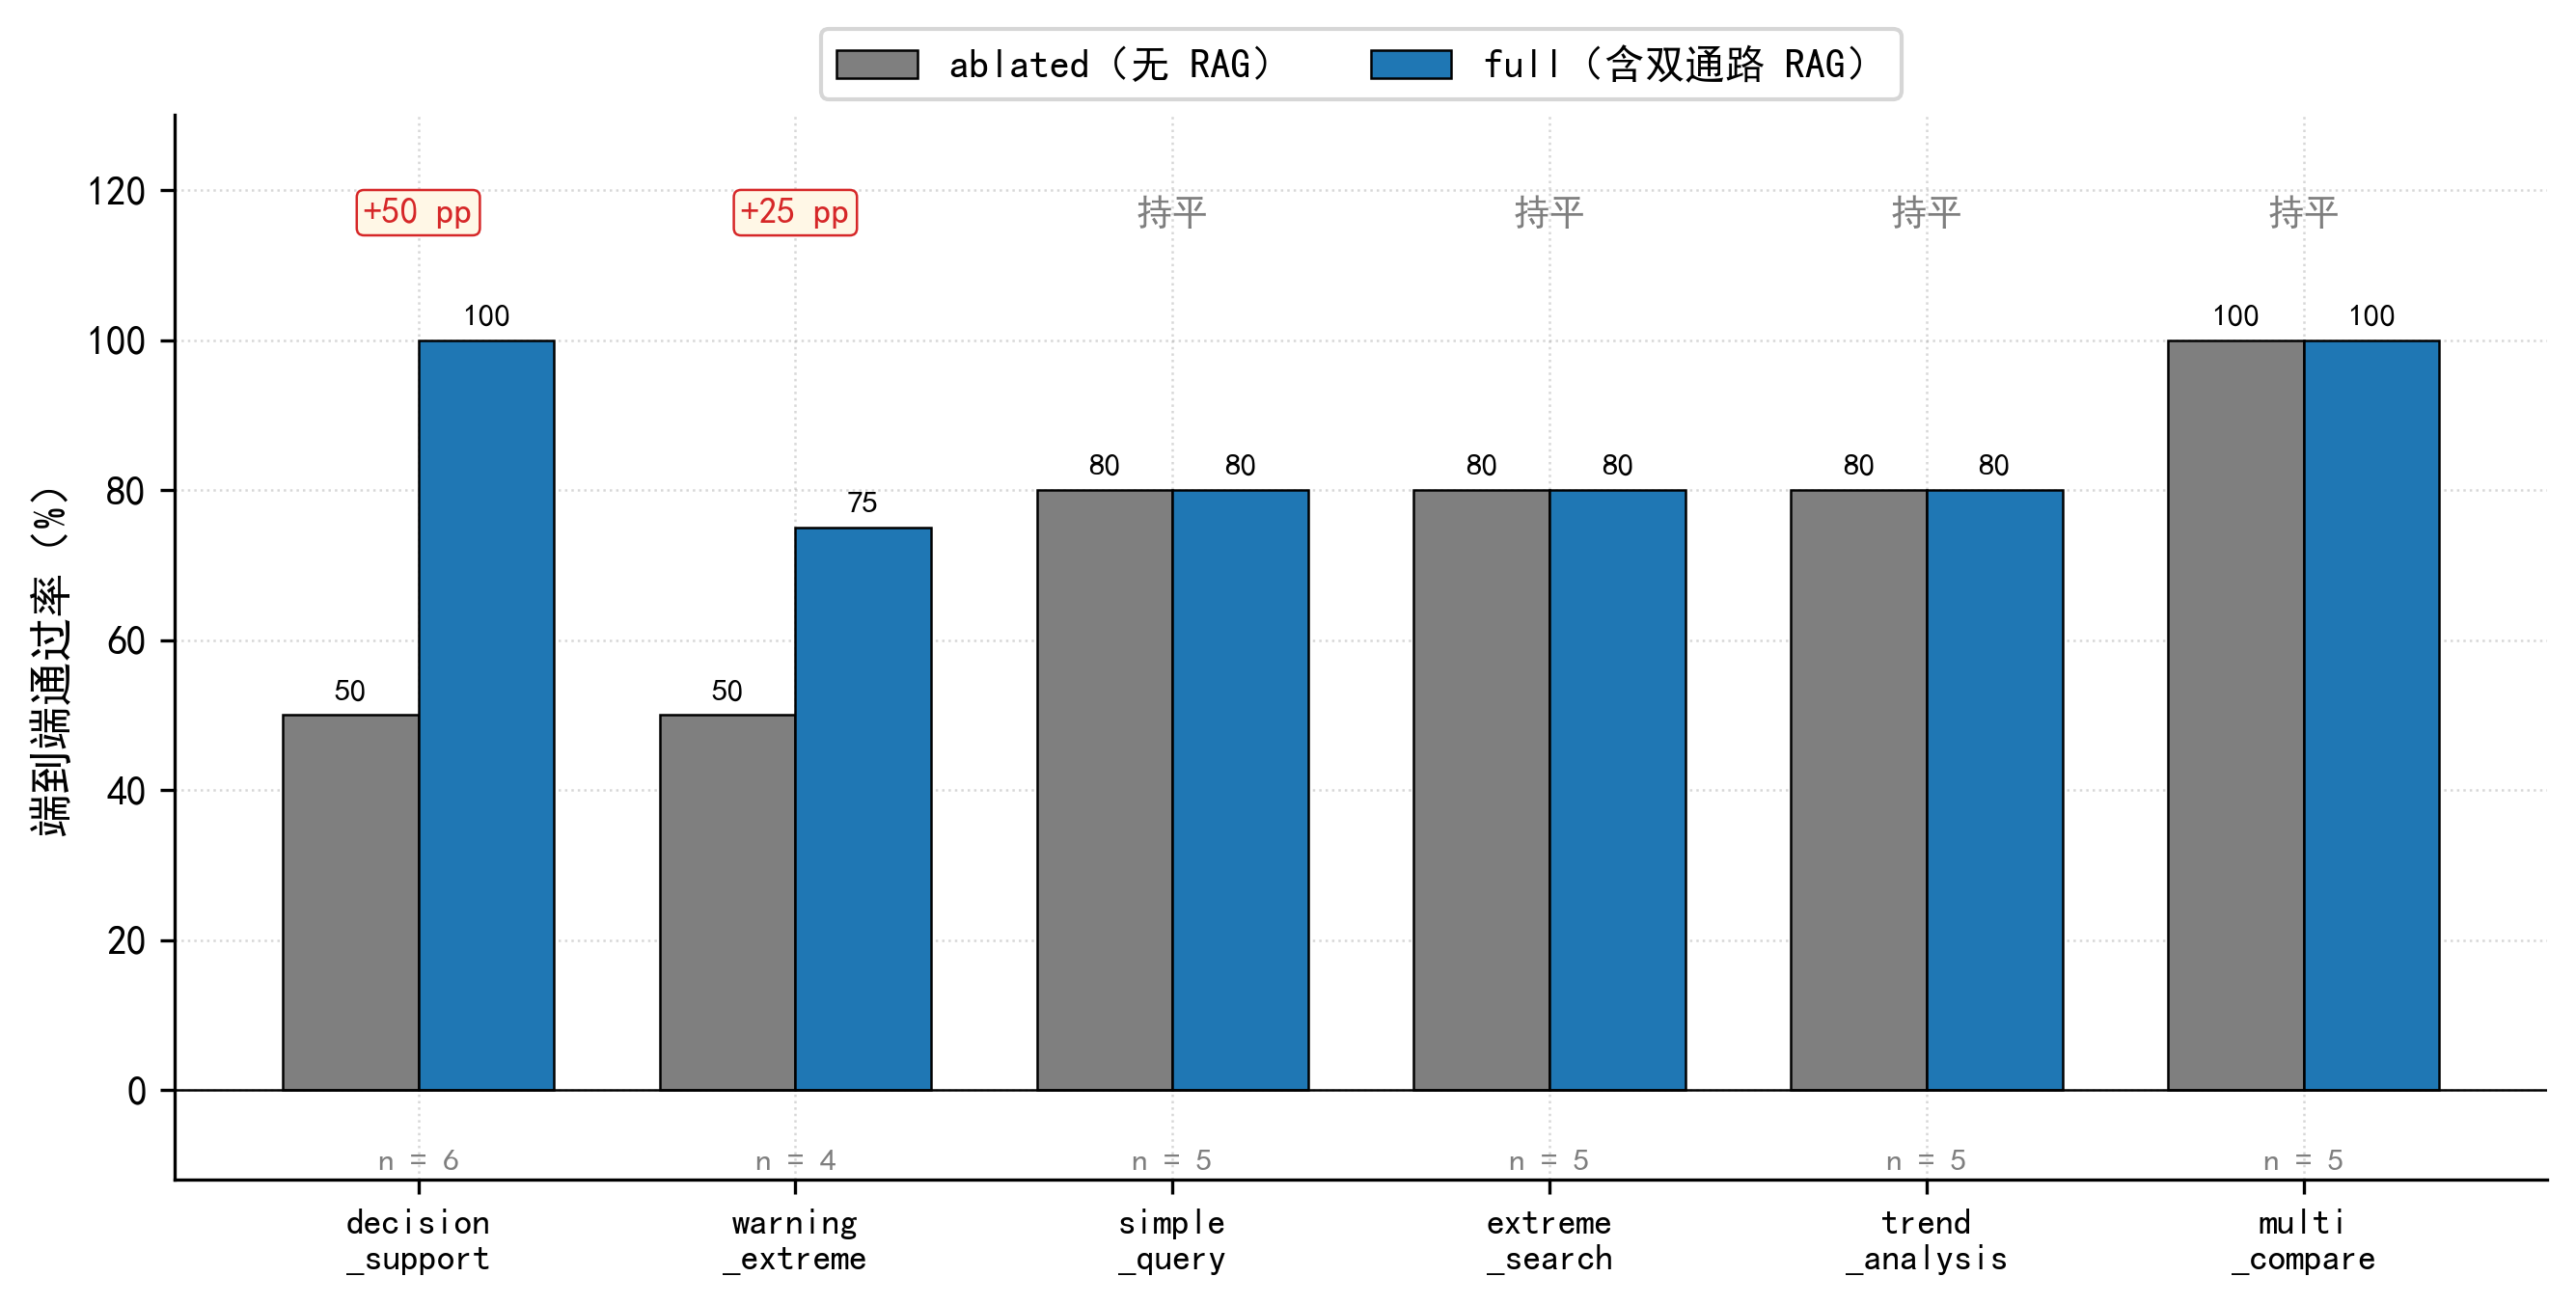
\includegraphics[width=0.95\linewidth]{figures/eval_5_5_e2e_by_category}
    \caption{端到端通过率按场景类别拆分：\texttt{ablated}（无 RAG）与 \texttt{full}（含双通路 RAG）双档对照（30 条用例）}
    \label{fig:e2e-by-category}
\end{figure}

\begin{table}[H]
    \centering
    \caption{端到端评测按场景类别拆分}
    \label{tab:e2e-by-category}
    \song\wuhao
    \begin{tabular}{lrccc}
        \toprule
        场景类别 & 用例数 & ablated & full & 差距 \\
        \midrule
        \texttt{decision\_\bk{}support} & 6 & 50.0\% & 100.0\% & $+50.0$ pp \\
        \texttt{warning\_\bk{}extreme} & 4 & 50.0\% & 75.0\% & $+25.0$ pp \\
        \texttt{simple\_\bk{}query} & 5 & 80.0\% & 80.0\% & 持平 \\
        \texttt{extreme\_\bk{}search} & 5 & 80.0\% & 80.0\% & 持平 \\
        \texttt{trend\_\bk{}analysis} & 5 & 80.0\% & 80.0\% & 持平 \\
        \texttt{multi\_\bk{}compare} & 5 & 100.0\% & 100.0\% & 持平 \\
        \bottomrule
    \end{tabular}
\end{table}

LLM-as-judge 4 维度评分见 \ref{sec:report-generation} 节
\reftab{tab:report-judge-summary}。差距集中在专业性维度的 $+0.37$，
事实性、完整性、流畅性三档接近持平甚至 \texttt{ablated} 档略胜。综合
分仅相差 0.04 是因为 Judge 等权平均稀释了专业性的差距。这一结果与
端到端通过率 13.4 个百分点的差距并不矛盾：通过率把该引用时必须引用
作为硬条件，而 Judge 综合分允许模型在事实性与流畅性上获得高分而对
专业性失分形成补偿。这两个指标分别从软性印象与硬性要求两个角度刻画
报告质量，共同反映双通路 RAG 的价值。

值得专门指出的两个失败用例。第一个是 \texttt{warning\_\bk{}001\_\bk{}rainstorm}
即 \ref{sec:report-generation} 节的暴雨判定案例：\texttt{ablated} 档
正确给出 50 mm 暴雨阈值数值但无引用源，\texttt{full} 档直接引用
GB/T 28592-2012 §4.1。第二个是 4 条 \texttt{full} 档失败用例的共性：
模型在 RAG 结果中确实拿到了相关分级阈值，但在最终报告生成时省略了
GB/T 编号。这一现象解释了为什么通路 B 单测 \texttt{citation} 真实性
已经达到 100\%，端到端集成后仍只达到 26.7\%。集成衰减效应是 ReAct
循环 \cite{ref18} 在最后报告生成步骤上的特有局限，单纯依赖 prompt
工程显式注入引用约束已经将端到端引用率从 0\% 提升到 26.7\%，但仍
未达到 100\%。具体改进方向包括引用强制注入、生成后自动校验、模型
微调三类，在 \ref{sec:future-work} 节展开。

到目前为止论文已积累 5 组实证：通路 A 检索 60 条 / Top-1 85\%、
通路 B 桥接 71 条 / \texttt{grade\_\bk{}id} 100\% / \texttt{citation}
真实性 100\%、意图理解 35 条 / 端到端 91.4\% / 角色 100\%、代码执行
18 条 / 数值准确率 +22.2 pp、端到端 30 条 / 任务完成率 +13.4 pp /
权威引用率 +26.7 pp。前 4 组是中间产物视角，第 5 组首次以最终用户
体验视角完成集成层验证。开题报告 §3.4 承诺的 5 项评测指标
\texttt{Acc\_\bk{}intent}、\texttt{F1\_\bk{}param}、\texttt{Acc\_\bk{}analysis}、
\texttt{Task\_\bk{}completion} 与报告生成质量至此全部完成实证支撑，与
Kim 等 \cite{ref1} 的多智能体气候 Agent 评测体系在覆盖维度上对齐。
